\documentclass[11pt]{article}

\usepackage{graphicx}
\usepackage{courier}

\title{TMD Documentation}
\author{Adam Yedidia}

\begin{document}
    
\maketitle

This document is intended for users who wish to learn how to program in TMD. For users who only want to know how to run or compile a TMD directory, without needing to create one of their own, information on how to do that is available in the \texttt{tmd\_readme.pdf} file. The video tutorial at the root of this repository also explains how to run or compile TMD directories. \\

The top-level representation is a program written in the TMD language, which is a language designed to give the user a simple interface with which to program a multi-tape, 3-symbol Turing Machine with a function stack. Each of the many tapes in the execution of the program is infinite in one direction. \\

TMD code can be processed in two ways. First, it can be \emph{interpreted}; that is, it can be directly evaluated line-by-line. This is generally done to verify a program's correct behavior, and to correct errors which would result in thrown exceptions in the interpreter but might lead to undefined behavior in the compiled Turing machine (because the compiled Turing machine is optimized for parsimony, whereas the interpreter need not be). \\

Second, TMD code can be \emph{compiled} down to a description of a single-tape, 2-symbol Turing machine. It is highly recommended, however, to first interpret any piece of TMD code before compiling it, because the interpreter is much better for catching programming errors. The compiler is general-purpose and not restricted to compiling the programs discussed in this thesis. It is optimized to minimize the number of states in the resulting Turing machine, not to make the resulting Turing machine time- or space-efficient. \\

A TMD program is contained in a directory. It is a collection of \emph{functions}, each of which contains a sequence of \emph{commands}. Each function is given its own file. Commands are separated by newlines. Each command is given its own line. \\

A TMD program also contains two special files which contain important information about the multi-tape Turing Machine: a file named {\tt functions.tff} and a file named {\tt initvar}. \\ 

What follows is a brief description of the syntax of the TMD language. A much more detailed description is available at~\cite{github}. The brief description contained here should be enough for a reader to gain a reasonable understanding of the programs written for this paper; any reader wishing to write her own programs is strongly encouraged read the more detailed documentation before proceeding.

\section{TMD Files}

Most of the logic contained within a TMD program lies in its TMD files, each of which describes one function in the program. TMD functions can make reference to the tapes in the machine and read the symbol under the head of each tape, much as a standard multi-tape TM can. In addition, TMD functions can call other TMD functions, pushing those functions to the top of the stack. Finally, TMD functions can return, popping themselves from the function stack. \\

A TMD function file is composed of four kinds of lines: an input line, calls to other functions, tape commands, and return statements. \\

TMD function files must use the extension \texttt{.tmd}.

\subsection{The Input Line}

Every TMD function file begins with an input line. TMD function files cannot contain more than one input line. The input line describes what tapes are going to be passed in as arguments to the function, and will therefore be readable and writeable within the function. An example of an input line might be: \\ \\
\texttt{input x y z}

\subsection{Labels}

Any line in a TMD function other than the input line may be preceded by a \emph{label}. A label takes the following form: \\ \\
~[alphanumeric string]\texttt{:} [line of code] \\

A label is an indicator attached to a line of code. Using tape commands, the line of code can be referenced in order to jump to the labelled line of code. The label can also be given a descriptive name that helps to explain the purpose of the line. This is perfectly legitimate even if the programmer has no intention of jumping to the line later; the addition of a label results in no additional states in the compiled program.

\subsection{Function Calls}

Function calls call a TMD function defined within the directory, placing the newborn function call at the top of the function stack with a new program counter of 0 (indicating that the first line of the called function should be the first to be read). The return address of the function call is the line following the function call. \\

Function calls have the following form: \\ \\
\texttt{function }[function name]([argument name]$)^*$ \\

When a function call is executed, the function that is described by the file [function name]\texttt{.tmd} is executed, starting with its top line. If no file [function name]\texttt{.tmd} exists within the program directory, an error is thrown at compile-time or upon interpreting the function call. \\ 

An example of a function call might be: \\ \\
\texttt{function add x y}

\subsection{Tape Commands}

Tape commands begin with a marker that indicates which tape is going to be used in the command. They then explain what to do if each possible symbol is read.

In TMD, there are three legal tape symbols; they are \texttt{1}, \texttt{E}, and \texttt{\_}. \texttt{\_} is the empty symbol (the only one which can appear an infinite number of times on any tape). Furthermore, in TMD, it is a requirement that each tape always have the form $\texttt{\_}(\texttt{1}|\texttt{E})^{+}(\texttt{\_})^{\infty}$ (here, the $(.)^+$ operation denotes repetition any positive number of times, and the $(.)^\infty$ operation denotes repetition an infinite number of times). This requirement is for ease of compilation down to a single-tape TM; later, when the TMD is compiled down a Turing machine and that Turing machine is searching the registers for a register that matches a specific ID, the search will assume that the register organization will alternate (identifier, value, identifier, value) and that a value will be represented as a ``chunk'' of 1's and E's. This is why the above requirement must be respected. \\

Tape commands have the following form: \\

\texttt{[}[variable name]\texttt{]} ([symbol read] \texttt{(} [list of reactions] \texttt{)}$)^*$ \\

The list of reactions is a series of words separated by commas and encompassed by parentheses. Different reactions are separated by semicolons. These reactions can include what direction to move, what symbol to write, and what line to jump to after execution. \\

The symbols \texttt{1}, \texttt{E}, and \texttt{\_} are used to denote what symbol to write on the tape after reading. The symbols \texttt{R}, \texttt{L}, and \texttt{-} are used to denote what direction the head should move after writing (with \texttt{R} indicating a move rightward, \texttt{L} indicating a move leftward, and \textrm{-} indicating a command to remain stationary). Any other string denotes a label, indicating a jump to the relevant label. Therefore, TMD programmers should not name their labels \textrm{R} (for example)! This will confuse the compiler. Additionally, TMD programmers should not put two conflicting reactions in the same command, such as two different move commands. \\

Any type of reaction that is excluded from a parenthetical will be presumed to be the default. The default for each type is: \\ \\
-Symbol written: whatever symbol was read. \\
-Head move direction: \texttt{-} (in other words, no move). \\
-Jump: go to the next line. \\

As an example, the reaction \texttt{1 (E, -, LABEL)} would indicate that in response to reading a \texttt{1} on the tape, an \texttt{E} should be written, the head should not move, and the next line of code to be executed should be labelled LABEL. It would have identical behavior to the reaction \texttt{1 (E, LABEL)}, because \texttt{-} is the default behavior for which direction to move the head. \\

An example of a full tape command might be the following: \\
\texttt{FIND\_E: [x] 1 (R, FIND\_E); E ()} \\

This tape command would indicate that on the tape named \texttt{x}, if a \texttt{1} is read off the tape, then a \texttt{1} should be written back onto the tape (because that is the default), the head should move right, and the line of code should be re-executed. If an \texttt{E} is read off the tape, then an \texttt{E} should be written back onto the tape, the head should not move, and execution should proceed to the next line of code (because those are the defaults). Because no reaction is provided in the case where a \texttt{\_} is read off the tape, an error will be thrown if that is the symbol that is read, both in interpretation and in the Turing machine that results from compilation. \\

It should be noted that while there is no difference between explicitly writing out the default and leaving it implied for head moves and for symbol writes (so, for example, a TMD program including the line \texttt{[x] 1 (1)} will compile to an identical machine as a program including the line \texttt{[x] 1 ()}), there \emph{is} a difference between explicitly writing out the default and leaving it implied for jumps. This difference manifests itself only in terms of parsimony and not in terms of behavior, and therefore is only visible when compiling the program, not when interpreting it (since during interpretation, only behavior matters). This is because while in the case of an explicit jump, the jump address must be written out onto the tape, there is a much shorter abbreviation for the default if it is simply a jump to the next line. Figure~\ref{fig:defaultjump} shows this case in more detail.

\begin{figure} 
\begin{center} 
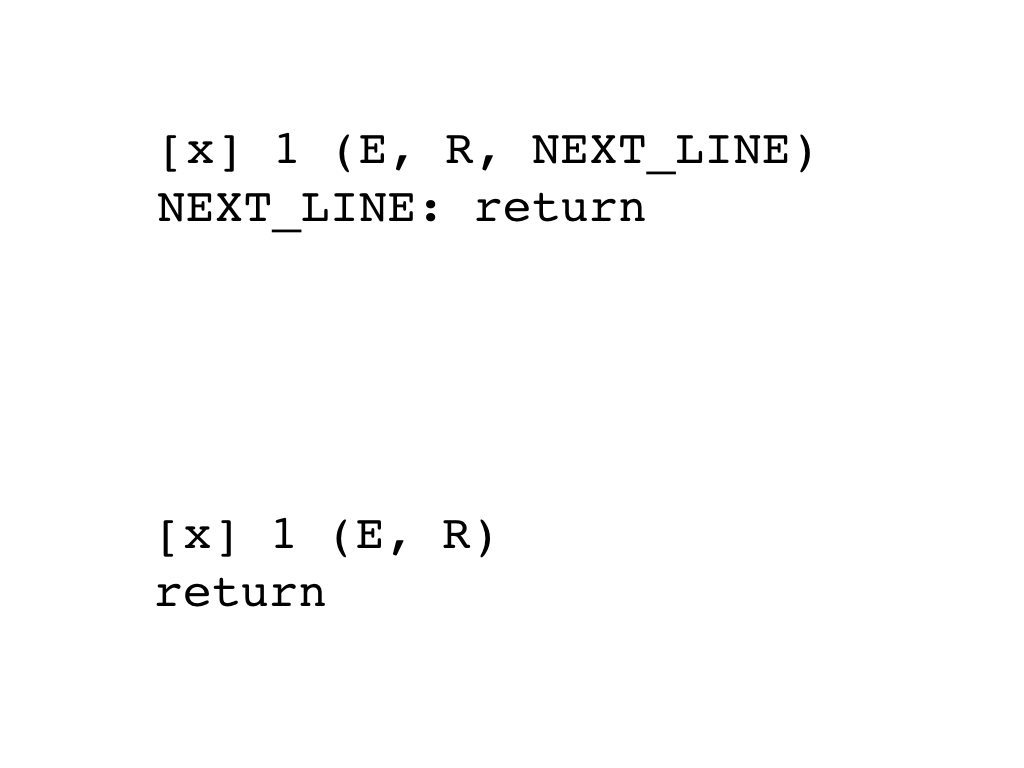
\includegraphics[scale=0.4]{figs/defaultjump.png}
\caption{This figure shows two code snippets. The two snippets will have identical behavior when interpreted or compiled, because the default is to jump to the next line. However, the bottom snippet will compile to a more parsimonious Turing machine (albeit one that behaves identically) because the compiler will know to use the default abbreviation for ``go to the next line,'' whereas in the top case the compiler will have to write out the jump address for the line labelled \texttt{NEXT\_LINE}. Therefore, it is recommended that programmers concerned with parsimony use the approach shown by the bottom snippet. \label{fig:defaultjump}} 
\end{center} 
\end{figure}

\subsection{Return Statements}

Return statements indicate the end of a function's execution. After a function returns, that function's call is popped off the function stack, and execution continues at the line of code following the line that called the function that just returned. If the function stack is empty, and there is no function to return to, the program halts. This will happen when the first function to be called finally returns. \\

Execution reaching the end of a function without returning will cause a runtime error. \\

\section{The \texttt{functions} File}

Every TMD directory must contain a file named \texttt{functions} (no extension). The \texttt{functions} file contains a list of every TMD function file in the directory that is used in the program. Note that not every TMD function file in the directory needs to be listed! If any such files are not listed, however, they must not be used in the program. If there is ever a call to a function not present in the \texttt{functions} file, there will be a runtime error (if the program is being interpreted) or a compilation error (if the program is being compiled). \\

When a TMD program is run, the first function to be called will be the function at the top of the \texttt{functions} file. \\

In the compiled TMD binary, the functions near the top of the \texttt{functions} file will be given shorter binary strings as names. Therefore, it is advantageous to put more frequently-called functions near the top of the \texttt{functions} file. (The Laconic-to-TMD converter does this automatically.)

\section{The \texttt{initvar} File}

Every TMD directory must contain a file named \texttt{initvar} (no extension). The \texttt{initvar} file contains a sequence of \texttt{1} and \texttt{E} symbols; this will be the sequence of symbols on each tape at initialization. So, for example, if the \texttt{initvar} file contains the string \texttt{11E1}, then each tape will be initialized with the values $\texttt{\_11E1}(\texttt{\_})^{\infty}$. \\

At initialization, every tape's head will begin just above the first non-\texttt{\_} symbol.

No \texttt{initvar} file may contain characters other than \texttt{1} and \texttt{E}. The \texttt{initvar} file cannot be empty.

\section{Example}

I have provided a simple example of a TMD directory to make it easier to understand what's going on. It can be found at \texttt{parsimony/src/tmd/tmd\_dirs/example\_tmd\_dir}. Before reading on, please navigate to this directory---I will make reference to its contents in this section. \\

What happens when this program is run? Well, to know where the program starts, we look at the \texttt{functions} file. The \texttt{functions} file lists two functions, \texttt{f} and \texttt{g}. To know how the program starts, we mostly care about which function is at the top of the list; in this case, that's \texttt{f}. Therefore, execution is going to start at the top of the file describing \texttt{f}. At the top of the file describing \texttt{f} we see the line ``\texttt{input a b c}''; because \texttt{f} is the first function, this tells us that our program execution will make use of three tapes, named \texttt{a}, \texttt{b}, and \texttt{c}, respectively. \\

We also need to know how each tape is initialized. In order to know that, we need to look at the \texttt{initvar} file. In this directory, the \texttt{initvar} file contains only the string ``\texttt{E}''; that tells us that every tape in the program is initialized to the value $\texttt{\_E\_}^\infty$. \\

Now we are ready to begin the program. Our three tapes contain an \texttt{E} symbol and are otherwise covered in \texttt{\_}'s. Our function stack begins with a single call to \texttt{f}. We look at the top command of \texttt{f.tmd}, ignoring the comment. It reads: ``\texttt{function g a}''. This indicates that the first thing we must do is call the function \texttt{g}, with the tape \texttt{a} as an argument. \\

This we do, placing a call to \texttt{g} at the top of the stack. Execution now proceeds from the top of \texttt{g}. We see from the input line of \texttt{g} that it takes one input, named \texttt{x}. We recognize that because \texttt{g} was called on the tape \texttt{a}, any references to \texttt{x} in the call to \texttt{g} are in fact going to read and modify \texttt{a}. \\

We look at the top command of \texttt{g}, ignoring the comment. It reads: ``\texttt{[x] E (1)}''. This indicates we are to read ``\texttt{x}'' (which we know to in fact refer to \texttt{a}) and read the symbol on it. If that symbol is an \texttt{E}, we will write a 1 onto the tape, keep the head stationary, and proceed to the next line; otherwise, we will throw an error (because no instructions are provided for how to handle symbols other than \texttt{E}). \\

In fact, all three tapes currently have a \texttt{E} symbol under the head, because that's how they were initialized. Thus, we read the \texttt{E} symbol from off \texttt{a}, replace it with a \texttt{1} symbol, and proceed to the next line. \\

The next line reads: ``\texttt{return}''. This tells us to pop the call to \texttt{g} off the stack and continue execution where we were in the function that called \texttt{g}. This leads us to the second command of \texttt{f}, which reads: ``\texttt{[b] 1 (RETURN); E ()}''. This tells us to read what is under the head on tape \texttt{b}, and if it's a \texttt{1} to go to the line of code labelled \texttt{RETURN} and otherwise to proceed to the next line of code. In either case, we don't change what's written on the tape, nor do we move the tape head. \\

Recall that at the moment, \texttt{a} has a \texttt{1} symbol, but both \texttt{b} and \texttt{c} are unchanged from when they were initialized. Therefore, we read a \texttt{E} symbol from off the tape; this tells us to proceed simply to the next line. \\

This is where things start to get a little bit confusing. The next line tells us to call \texttt{f} recursively, on a permutation of its own inputs. This we do, placing a new call to \texttt{f} on top of the old call to \texttt{f}. We look at the input line of \texttt{f}; it says ``\texttt{input a b c}''. This indicates to us that in this function call, the first argument to \texttt{f} will be called ``\texttt{a}'', the second ``\texttt{b}'', and the third ``\texttt{c}''. Recall that when we called \texttt{f} from within the original function, we called \texttt{f} on \texttt{b}, \texttt{c}, and \texttt{a}, in that order. This means that in the new function call, ``\texttt{a}'' will refer to the first argument of the function call, or \texttt{b}. Similarly, ``\texttt{b}'' will refer to \texttt{c}, and ``\texttt{c}'' to \texttt{a}. \\

With that in mind, let's begin executing the new call to \texttt{f}. The first command is a command to call \texttt{g} on ``\texttt{a}'', which in fact refers to \texttt{b}. The function \texttt{g} reads \texttt{b}, and finding an \texttt{E} under the head, replaces it with a \texttt{1} and returns. Our three tapes \texttt{a}, \texttt{b}, and \texttt{c} now contain a \texttt{1}, a \texttt{1}, and an \texttt{E}, respectively. \\

The next command tells us to read the symbol on ``\texttt{b}'', which in fact refers to \texttt{c}. Given that \texttt{c} still contains an \texttt{E}, we proceed simply to the next line. The next line tells us to make a \emph{new} call to \texttt{f}, with ``\texttt{b}'' (actually \texttt{c}) as the first argument, ``\texttt{c}'' (actually \texttt{a}) as the second argument, and ``\texttt{b}'' (actually \texttt{c}) as the third argument. \\

Still following? To know how to interpret which names point to which tapes in the newborn call to \texttt{f}, we look its input line; it says (still!) ``\texttt{input a b c}''. This indicates to us that in this new function call, the first argument to \texttt{f} will be called ``\texttt{a}'', the second ``\texttt{b}'', and the third ``\texttt{c}''. But remember that in the function that called this one, \texttt{c} was the first argument, \texttt{a} was the second argument, and \texttt{b} the third! Therefore, in this newest function call, ``\texttt{a}'' will refer to \texttt{c}, ``\texttt{b}'' to \texttt{a}, and ``\texttt{c}'' to \texttt{b}. \\

That was one of the more confusing paragraphs that I've written in my lifetime, so let's take a step back. We have three tapes, \texttt{a}, \texttt{b}, and \texttt{c}, that contain \texttt{1}, \texttt{1}, and \texttt{E}, respectively. Our function stack contains three calls to \texttt{f}. Across those function calls, the names ``\texttt{a}'', ``\texttt{b}'', ``\texttt{c}'' refer to different things. In the bottom call, the names (``\texttt{a}'', ``\texttt{b}'', ``\texttt{c}'') refer to (\texttt{a}, \texttt{b}, \texttt{c}). In the middle call, the names (``\texttt{a}'', ``\texttt{b}'', ``\texttt{c}'') refer to (\texttt{b}, \texttt{c}, \texttt{a}). And in the top call, the names (``\texttt{a}'', ``\texttt{b}'', ``\texttt{c}'') refer to (\texttt{c}, \texttt{a}, \texttt{b}). \\

Okay. Now we can start executing the top call to \texttt{f}. The top command tells us to run \texttt{g} on ``\texttt{a}'' (actually \texttt{c}). The function \texttt{g} reads \texttt{c}, and finding an \texttt{E} under the head, replaces it with a \texttt{1} and returns. Now our three tapes all contain a \texttt{1}. Next, we execute the command ``\texttt{[b] 1 (RETURN); E ()}''. This tells us to read ``\texttt{b}'' (actually \texttt{a}). Upon reading \texttt{a}, we see that it contains a \texttt{1}. We are told to jump to the line of code labelled \texttt{RETURN}. The line of code labelled \texttt{RETURN} says ``\texttt{return}''; thus, we pop the top call to \texttt{f} off the stack, and we continue execution where we were in the function that called \texttt{f}. \\

The function that called \texttt{f} was itself a call to \texttt{f}, but with a different mapping from tape names to actual tapes. The line after the function call is the last line of \texttt{f}, which reads ``\texttt{return}''. Thus, this middle call to \texttt{f} is also popped off the stack, and we continue execution in the original call to \texttt{f}. \\

The line we were on in the original call to \texttt{f} was also the last line of \texttt{f}. It reads \texttt{return}. Therefore, we pop it off the stack too. \\

Now the stack is empty. If ever the stack is empty, execution halts. Therefore, we halt here, leaving the three tapes containing a \texttt{1}.

For a pictorial representation of what happened here, navigate to \texttt{parsimony/src/tmd/tmd\_meta/} and enter the command \texttt{python tmd\_interpreter.py example\_tmd\_dir}. Then, read the output file \texttt{example\_tmd\_dir\_history.txt}, found in the \texttt{parsimony/src/tmd/tmd\_histories/} directory.

\end{document}